% !TEX options=--shell-escape
	\documentclass{article}
	\usepackage{amsmath,amssymb}
	\usepackage[inline]{enumitem}
	\usepackage{blindtext}
	\usepackage{booktabs}
	\usepackage{graphicx}
	\usepackage{xcolor}
	\usepackage[vmargin = 1.5in, top = 1in, bottom = 1.2in, letterpaper]{geometry}
	\usepackage{listings}
	\usepackage{courier}
	\usepackage{multicol}
	\usepackage{multirow}
	\usepackage{bm}
	\usepackage[labelformat=simple]{subcaption}
	\renewcommand\thesubfigure{(\alph{subfigure})}
	\usepackage{minted}
	\usepackage{fvextra}
	\definecolor{bg}{rgb}{0.95,0.95,0.95}
	\newminted{r}{mathescape, breaklines, linenos = true, bgcolor = bg}
	\usemintedstyle{tango}
	% \lstset{
	% basicstyle = \small\tt,
	% keywordstyle = \tt\color{blue},
	% commentstyle = \it\color[cmyk]{1,0,1,0},
	% stringstyle = \tt\color[RGB]{128,0,0},
	% %frame = single,
	% backgroundcolor = \color[RGB]{245,245,244},
	% breaklines,
	% extendedchars = false,
	% xleftmargin = 2em,
	% xrightmargin = 2em,
	% aboveskip = 1em,
	% tabsize = 4,
	% showspaces = false
	% }
	\newcommand\inner[2]{\left\langle{#1},{#2}\right\rangle}
	\DeclareMathOperator{\Corr}{Corr}
	\DeclareMathOperator{\Cov}{Cov}
	\DeclareMathOperator{\Var}{Var}
	\DeclareMathOperator{\E}{E}



	\begin{document}
	
	% \newfontfamily\courier{Courier New}

	
	\title{STAT 501 Homework 4}
	\author{Multinomial}
	\maketitle
	
	\begin{enumerate}[leftmargin = 0 em, label = \arabic*., font = \bfseries]
	\item 
	\begin{enumerate}
		\item 
		We choose to plot the radial visualization to see any difference between the regions and sub-regions.
		\begin{rcode}
#Multinomial 
##Problem 1
#a) Radial visualization
library(lattice)
require(dprep)
olive <- read.table("http://maitra.public.iastate.edu/stat501/datasets/olive.dat", header=T)
olive
colnames(olive) <- c("Regions", "CH1", "CH2", "CH3", "CH4", "CH5","CH6","CH7","CH8")
names(olive)
oil<- as.factor(olive$Regions)

# Use codes from Canvas
source("radviz2d.R")
# Display the radial visualization plot 
radviz2d(dataset = cbind(olive[,-1], oil), name = "Regions")

# sub-regions R1
olive_R1 <- olive[olive$Regions %in% 1:4,]
radviz2d(dataset = cbind(olive_R1[,-1], as.factor(olive_R1$Regions)), name = "R1")

# sub-region  R2
olive_R2 <- olive[olive$Regions %in% 5:6,]
radviz2d(dataset = cbind(olive_R2[,-1], as.factor(olive_R2$Regions)), name = "R2")

# sub-region  R3
olive_R3 <- olive[olive$Regions %in% 7:9,]
radviz2d(dataset = cbind(olive_R3[,-1], as.factor(olive_R3$Regions)), name = "R3")
		\end{rcode}
		The plots are shown in Figure~\ref{Regions} and Figure~\ref{subregions}.
		\begin{figure}[!htb]
			\centering
			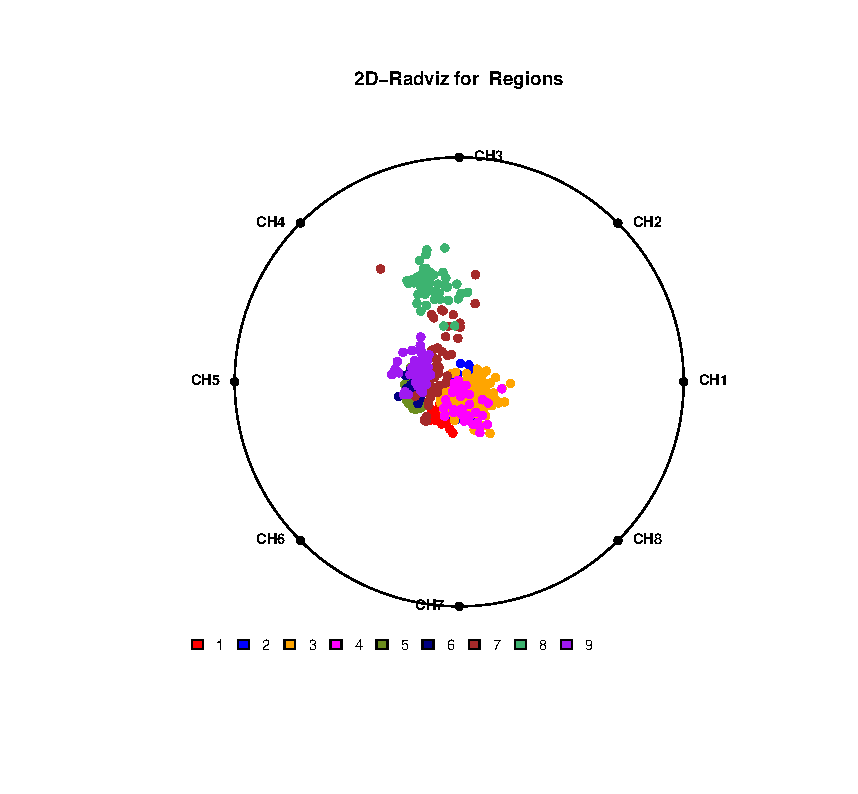
\includegraphics[width = 0.5\textwidth]{Regions.eps}
			\caption{Radial Visualization for all regions}
			\label{Regions}
		\end{figure}


        \begin{figure}
        \centering
          \begin{subfigure}[b]{.33\textwidth}
            \centering
            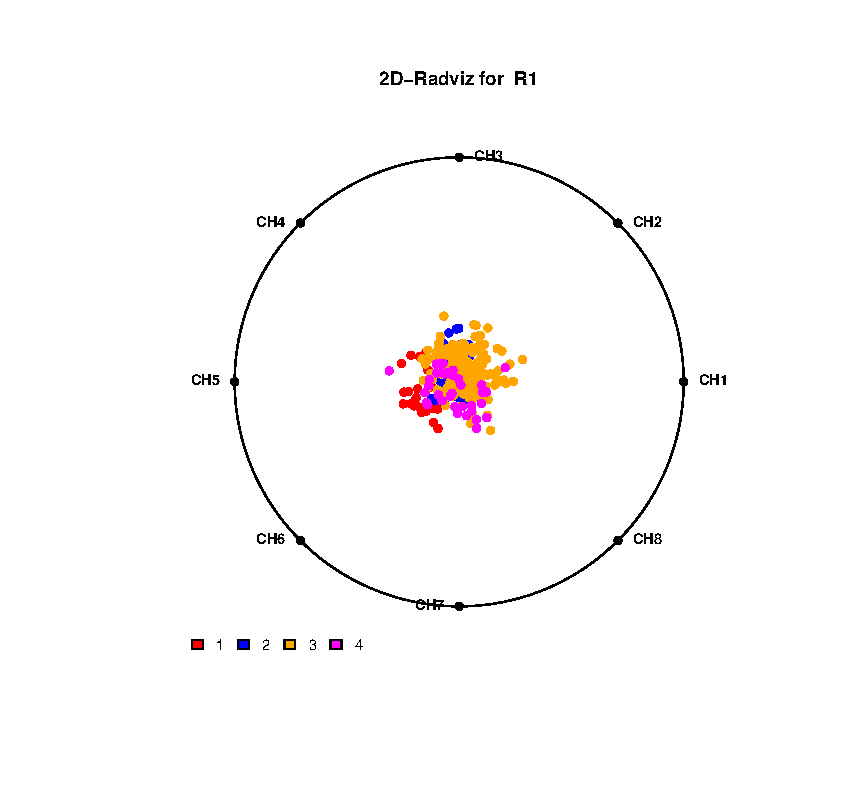
\includegraphics[width = \textwidth]{R1.eps}
            \caption{Region 1}
            \label{R1}
          \end{subfigure}%
          \begin{subfigure}[b]{.33\textwidth}
            \centering
            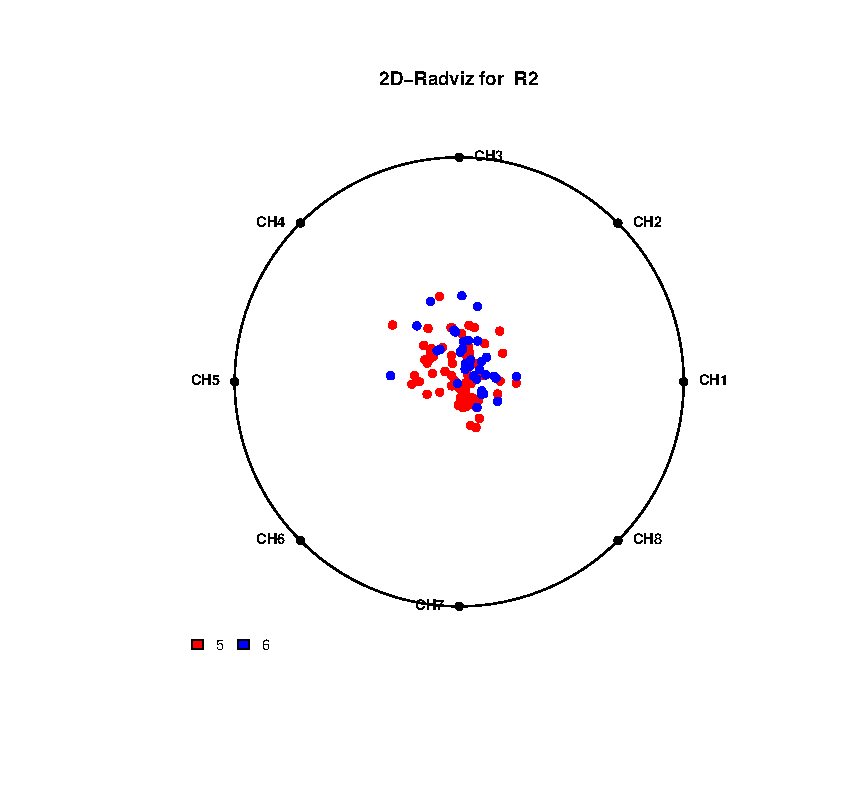
\includegraphics[width = \textwidth]{R2.eps}
            \caption{Region 2}
            \label{R2}
          \end{subfigure}%
           \begin{subfigure}[b]{.33\textwidth}
            \centering
            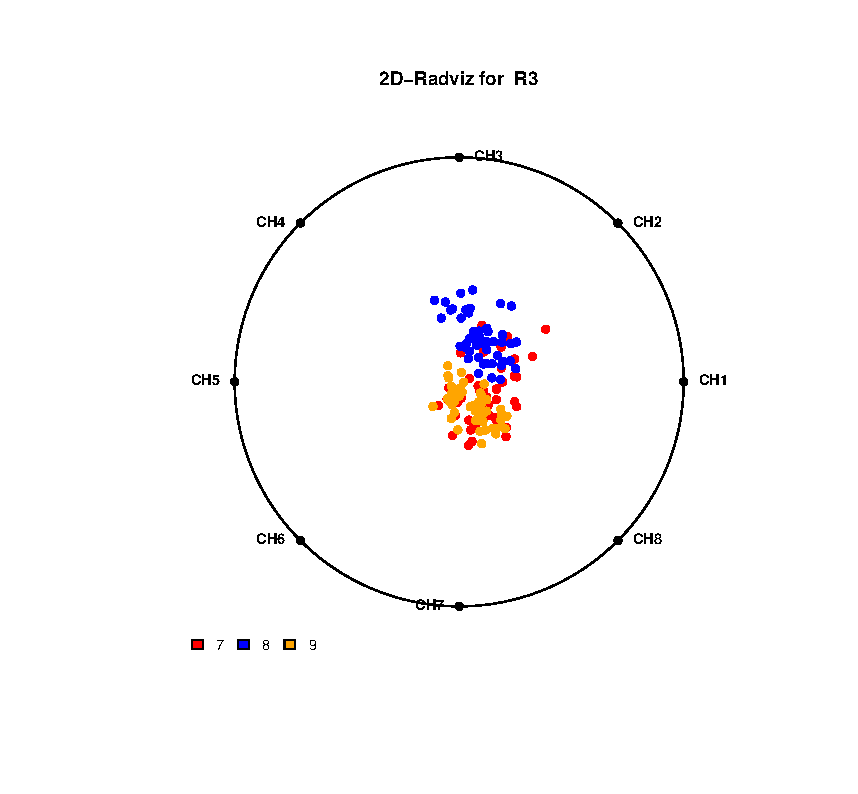
\includegraphics[width = \textwidth]{R3.eps}
            \caption{Region 3}
            \label{R3}
            \end{subfigure}
          \caption{Radial Visualization for sub-regions}\label{subregions}
\end{figure}

\newpage
The plot that contains all nine regions does not reveal exact difference between chemical components
of olive oil except component CH8. The second plot for sub-region 1 shows that all chemical components have quite same pattern.
The third plot for sub-region 2 indicates much overlap of chemical components. The plot for   sub-region 3 reveals the exact differnce between 
CH8, CH7 and CH9. If we compare three sub-regions, the chemical components behave differenly in each case. Among visualization methods, radial visualisation  might be effective since some other methods show only overall view of the chemical components.


	\item 
	\begin{enumerate}
		\item 
	In Regions 2, we calculate the correlation matrix for each of the two sub-regions:
	\begin{rcode}
#b) Choose the R2
#i) Calculate the correlation matrix of the two sub-regions
cor(olive_R2[olive_R2$Regions == 5, -1])
cor(olive_R2[olive_R2$Regions == 6, -1])
	\end{rcode}
	The results are:
	For Area 5:
	\begin{rcode*}{fontsize = \tiny}
            CH1         CH2         CH3         CH4         CH5        CH6         CH7         CH8
CH1  1.00000000 -0.25401254 -0.22343243 -0.34906506 -0.41062951  0.1668259 -0.03085139 -0.10589148
CH2 -0.25401254  1.00000000  0.15994615 -0.06232554  0.11648748  0.1587715  0.10500427  0.13394123
CH3 -0.22343243  0.15994615  1.00000000 -0.24736894  0.08986342 -0.3458010 -0.29500434 -0.04184051
CH4 -0.34906506 -0.06232554 -0.24736894  1.00000000 -0.38972482  0.1767836  0.13928597  0.01336267
CH5 -0.41062951  0.11648748  0.08986342 -0.38972482  1.00000000 -0.3416671 -0.08799411  0.03397236
CH6  0.16682592  0.15877145 -0.34580096  0.17678361 -0.34166707  1.0000000  0.45678706 -0.10181956
CH7 -0.03085139  0.10500427 -0.29500434  0.13928597 -0.08799411  0.4567871  1.00000000 -0.03620758
CH8 -0.10589148  0.13394123 -0.04184051  0.01336267  0.03397236 -0.1018196 -0.03620758  1.00000000
	\end{rcode*}
	For Area 6:
	\begin{rcode*}{fontsize = \tiny}
             CH1         CH2         CH3        CH4         CH5          CH6         CH7         CH8
CH1  1.000000000  0.11900039  0.08786970 -0.7994401  0.42188660 -0.007466556  0.33270138  0.40508513
CH2  0.119000387  1.00000000  0.40954913 -0.1868781 -0.17723037 -0.049145339  0.12964611 -0.03710676
CH3  0.087869701  0.40954913  1.00000000 -0.2811107 -0.01414057 -0.399135258  0.14357073  0.19619085
CH4 -0.799440133 -0.18687810 -0.28111067  1.0000000 -0.79232090  0.151300451 -0.60573225 -0.36134336
CH5  0.421886601 -0.17723037 -0.01414057 -0.7923209  1.00000000 -0.182269052  0.53905745  0.22800013
CH6 -0.007466556 -0.04914534 -0.39913526  0.1513005 -0.18226905  1.000000000  0.06465175  0.04913952
CH7  0.332701378  0.12964611  0.14357073 -0.6057323  0.53905745  0.064651746  1.00000000  0.24163350
CH8  0.405085132 -0.03710676  0.19619085 -0.3613434  0.22800013  0.049139516  0.24163350  1.00000000
	\end{rcode*}
	And then we display the correlation matrix side-by-side as in Figure~\ref{corrplot}.
	\begin{rcode}
source("plotcorr.R")
par(mfrow = c(1,2))
plot.corr(xx = olive_R2[olive_R2$Regions == 5, -1])
plot.corr(xx = olive_R2[olive_R2$Regions == 6, -1]) 
	\end{rcode}
	\begin{figure}[!htb]
		\centering
		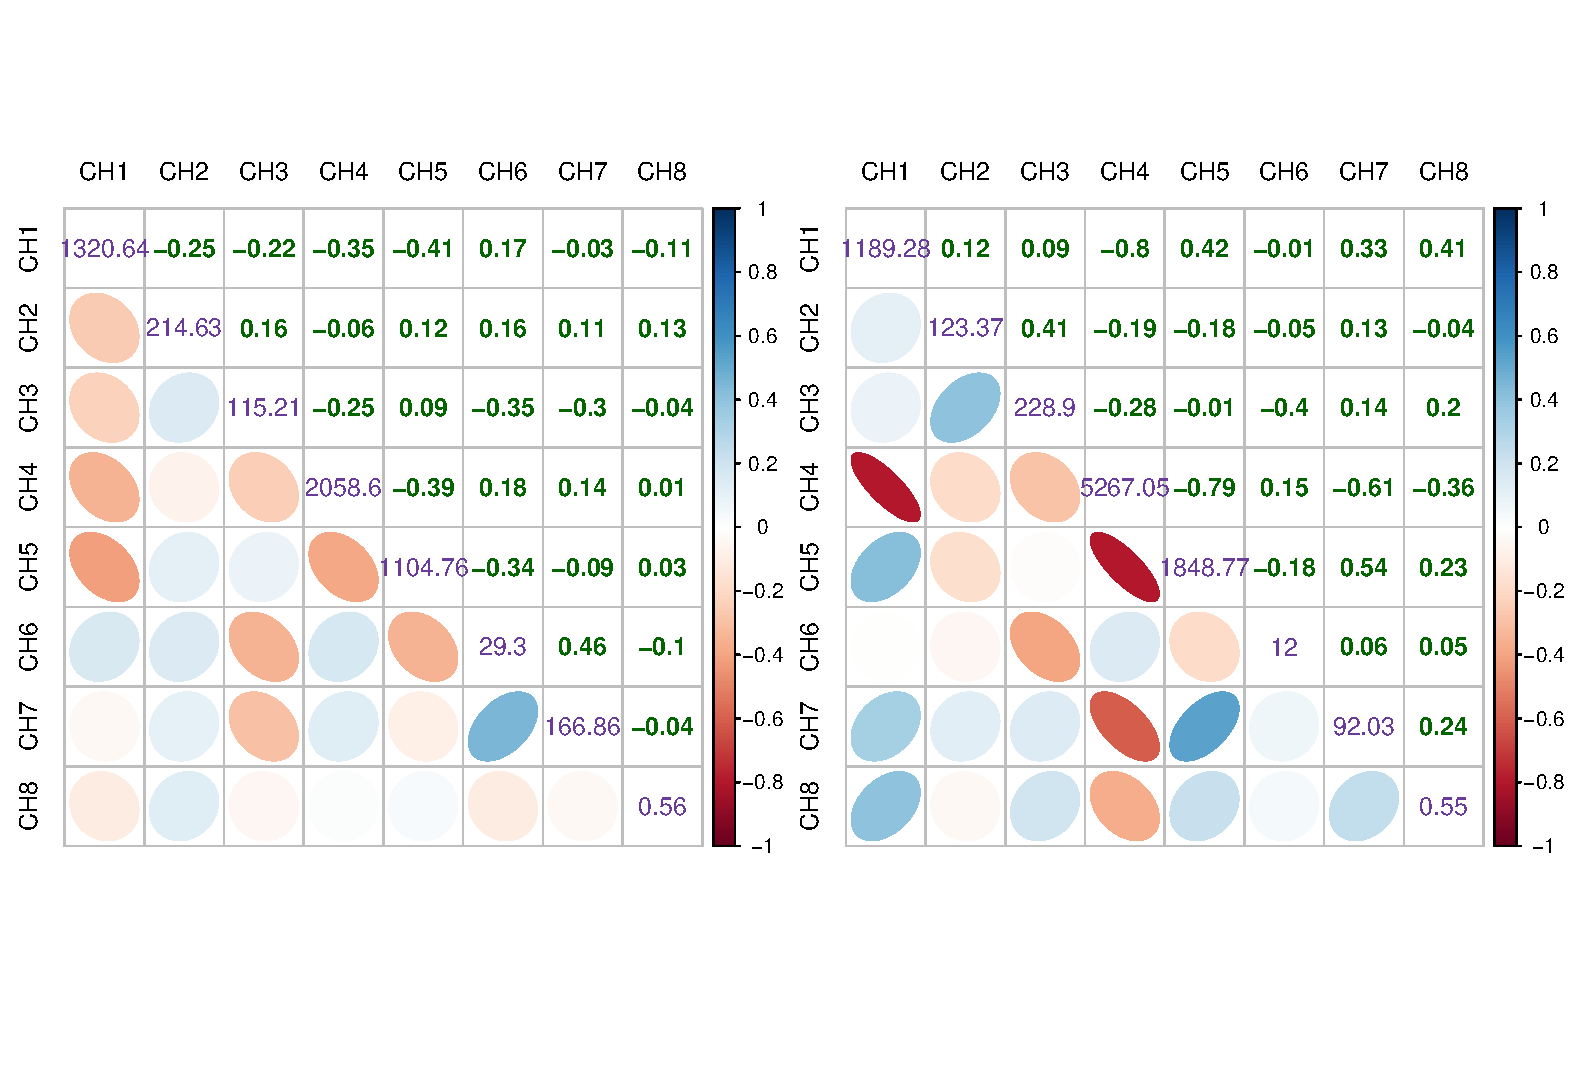
\includegraphics[width = \textwidth]{corrplot.eps}
		\caption{Correlation matrix display for Area 5 and Area 6}
		\label{corrplot}
	\end{figure}

According to the plots for Area 6, the correlation between CH4 and CH1, CH5 and CH4, CH4 and CH7 as well as CH5 and CH7 much strong than in Area 5.
In addition, the realtionship between CH1 and CH5 in Area 6 has a positive sign, however, in Area 5 is a negtaive.
Overall, we can conclude that chemical components in Area 6 hihgtly correlated than in Area 5.

\item 
Compare the marginal stadard deviations directly as well as with parallel coordinate plots:
\begin{rcode}
#ii) Compare marginal standard deviations
require(ggplot2)
require(GGally)
require(RColorBrewer)
source("parcoordplot.R")

SD_5<-sapply(olive_R2[olive_R2$Regions == 5, -1], FUN = sd)
SD_6<-sapply(olive_R2[olive_R2$Regions == 6, -1], FUN = sd)
# parallel coordinate plots
parcoordplot(xx =olive_R2[,-1] ,cl = as.factor(olive_R2$Regions),FUN=mean,alpha = 0.2)
\end{rcode}
And for Area 5, marginal standard deviations are:
\begin{rcode*}{fontsize = \footnotesize}
       CH1        CH2        CH3        CH4        CH5        CH6        CH7 
36.3406228 14.6501181 10.7336638 45.3717550 33.2379244  5.4126366 12.9173966 
       CH8
0.7493587
\end{rcode*}
For Area 6:
\begin{rcode*}{fontsize = \footnotesize}
      CH1       CH2       CH3       CH4       CH5       CH6       CH7
34.485916 11.107259 15.129554 72.574426 42.997291  3.464375  9.593243
      CH8 
 0.739830 
\end{rcode*}

The parallel coordinate plots as in Figure~\ref{parcoord}.

\begin{figure}[!htb]
	\centering
	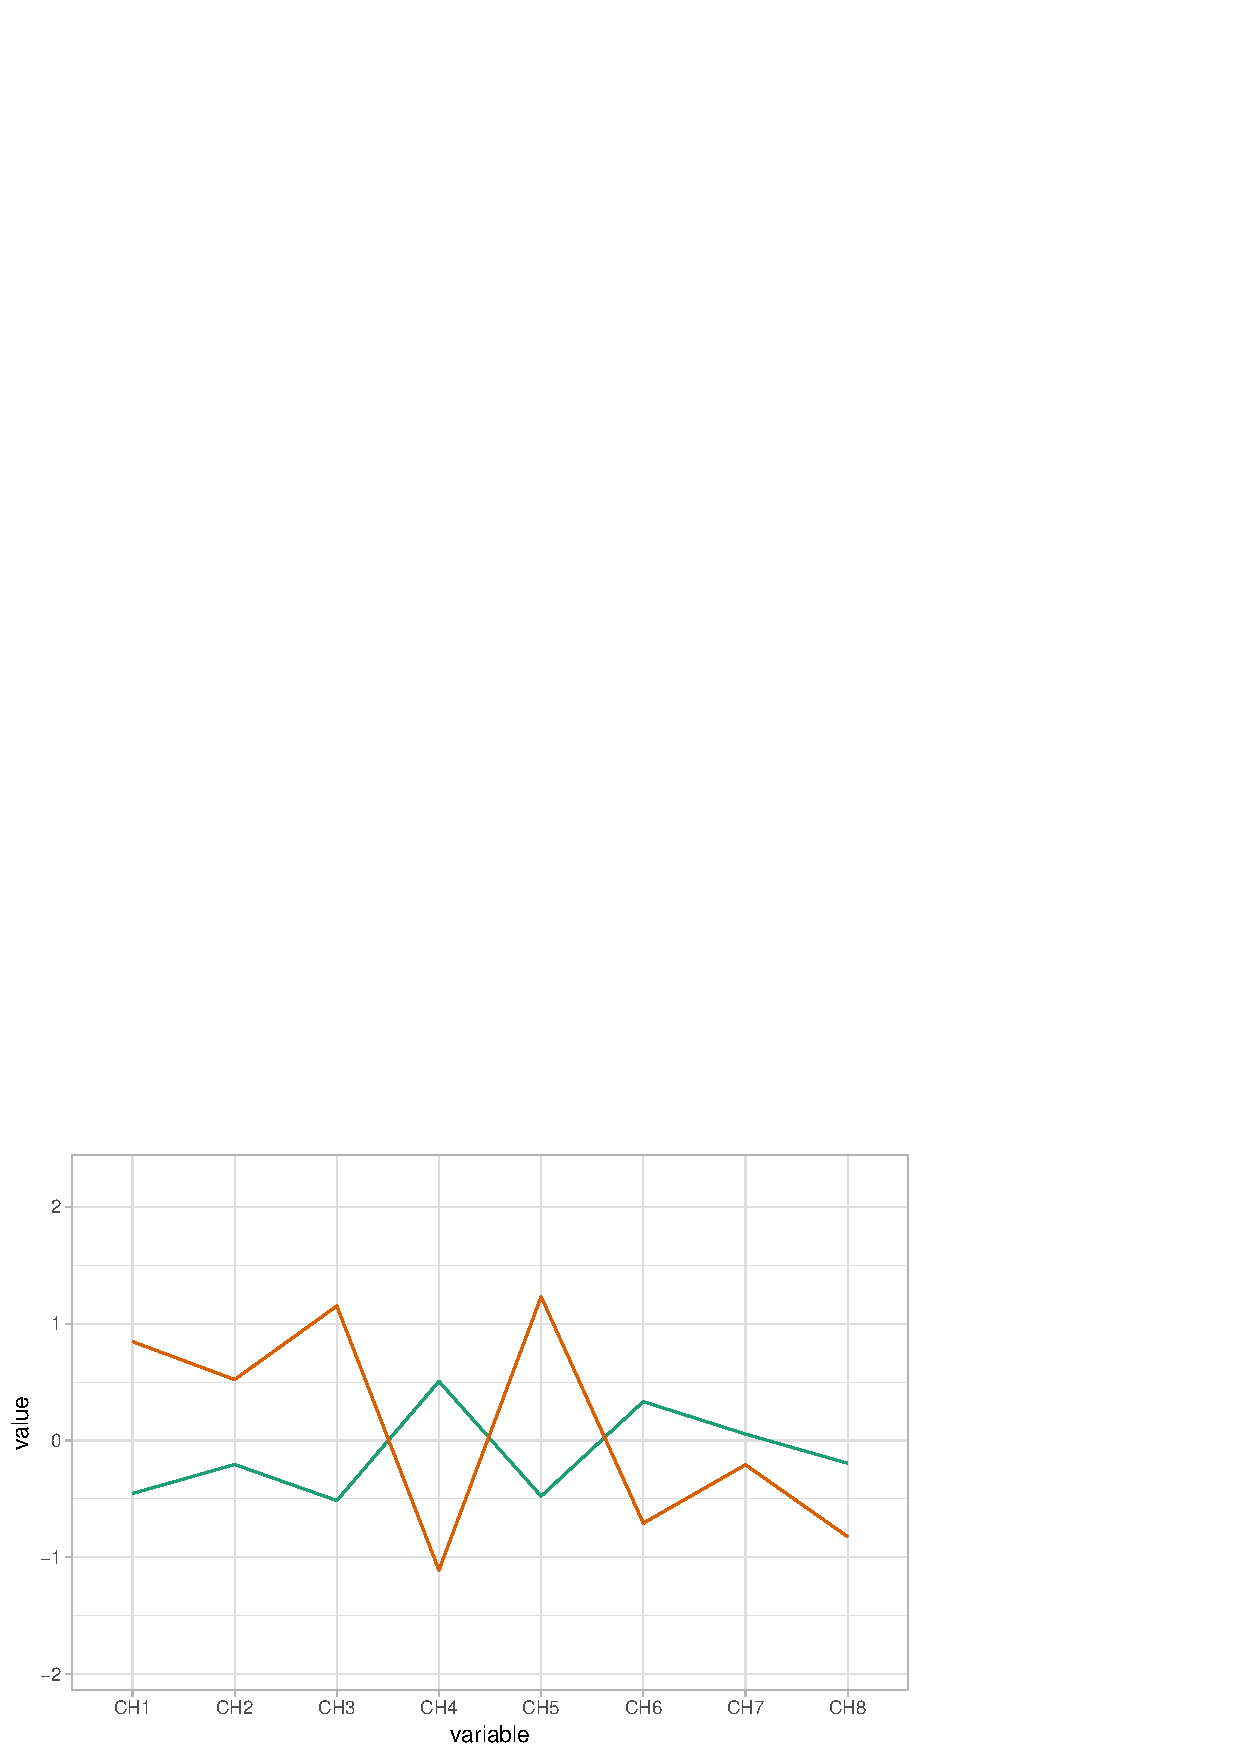
\includegraphics[width = 0.8\textwidth]{parcoord.jpeg}
	\caption{Parallel coordinate plots for Area 5 and Area 6}
	\label{parcoord}
\end{figure}

The standard deviation for Area 5 higher for CH1,CH2, CH7 and CH8 than in Area 6, however other 
the standard deviations of other chemical components are lower.

\item Test for difference in dispersions among the two groups
\begin{rcode}
#iii) Test for difference in dispersions among the two groups

source("BoxMtest-2.R")

BoxMTest(X = olive_R2[,-1], cl = as.factor(olive_R2$Regions))

\end{rcode}
The result is
\begin{rcode}
[1] 2
------------------------------------------------
 MBox Chi-sqr. df P
------------------------------------------------
  109.5204    98.3550          36       0.0000
------------------------------------------------
Covariance matrices are significantly different.
$MBox
       5 
109.5204 

$ChiSq
       5 
98.35502 

$df
[1] 36

$pValue
           5 
1.069438e-07 
\end{rcode}
With small p-value we conclude that there is significant evidence that the dispersions are different.

\item Test for normality
\begin{rcode}
#iv) Test for normality
source("testnormality.R")

 testnormality(X=olive_R2[olive_R2$Regions == 5, -1])
 testnormality(X=olive_R2[olive_R2$Regions == 6, -1])
\end{rcode}
The p-value for Area 5 is \textbf{1.743735e-06} and for Area 6 is \textbf{0.3706021}. The test result shows that for the Area 6 we can conclude multivariate normality is reasonable, but for Area 5 not.

\item Hotelling's $T^2$ test:
\begin{rcode}
library(ICSNP)
 T2test <- HotellingsT2(X = olive_R2[olive_R2$Regions == 5, -1], Y = olive_R2[olive_R2$Regions == 6, -1])
 T2test
 df1 <- T2test$parameter['df1']
 df2 <- T2test$parameter['df2']
 T2stat <- T2test$statistic/df2*(df1 + df2 - 1)*df1
 T2stat
\end{rcode}
The result of test is
\begin{rcode}
	#Hotelling's two sample T2-test

data:  olive_R2[olive_R2$Regions == 5, -1] and olive_R2[olive_R2$Regions == 6, -1]
T.2 = 112.41, df1 = 8, df2 = 89, p-value < 2.2e-16
alternative hypothesis: true location difference is not equal to c(0,0,0,0,0,0,0,0)
\end{rcode}
and p-value is less than \textbf{2.2e-16}, by adjust the result the true statistic
\[T^2 = \bf 969.9727\]
With small p-value we conclude that the two mean vectors are different for Area 5 and Area 6.

\item We do 8 individual t-tests for 8 chemicals and adjust the p-value with Bonferroni and FDR.
\begin{rcode}
 #vi) Provide individual t-tests
 
 tp_value<-function(X, cl){
   class <- levels(cl)
   return(t.test(X[cl == class[1]], X[cl == class[2]], var.equal = T)$p.value)
 }
 
 p_vals <- sapply(olive_R2[,-1], tp_value, cl = as.factor(olive_R2$Regions))
 
 p.adjust(p_vals, method = "bonferroni")
 p.adjust(p_vals[order(p_vals)], method = "fdr")
\end{rcode}

The adjusted p-values with Bonferroni:
\begin{rcode*}{fontsize=\footnotesize}
         CH1          CH2          CH3          CH4          CH5          CH6 
5.973326e-06 2.176220e-01 9.174890e-16 6.631503e-40 1.023099e-45 3.834440e-05  
         CH7          CH8 
1.000000e+00 1.000000e+00 
\end{rcode*}
The adjusted p-values with FDR:
\begin{rcode*}{fontsize=\footnotesize}
         CH5          CH4          CH3          CH1          CH6          CH2
1.023099e-45 3.315752e-40 3.058297e-16 1.493332e-06 7.668880e-06 3.627033e-02  
         CH7          CH8 
5.459712e-01 5.720031e-01 
\end{rcode*}
From these two adjusted p-values, we conclude that there is no significant differences in chemical 7 and 8 between Area 5 and 6, but there is differences in other chemical components.

\newpage
 \item Draw 95\% confidence ellipses, the ellipses are shown in Figure~\ref{ellips}.
 \begin{rcode}
 #vii) Draw 95% Confidence ellipses
 library(car)
 dataEllipse(olive_R2$CH5, olive_R2$CH6, groups = as.factor(olive_R2$Regions), levels=0.95, xlab = "CH5", ylab = "CH6", col = c("red", "blue"), ylim = c(10, 45), group.labels = c("A5", "A6"))
  \end{rcode} 
 \begin{figure}[!htb]
 	\centering
 	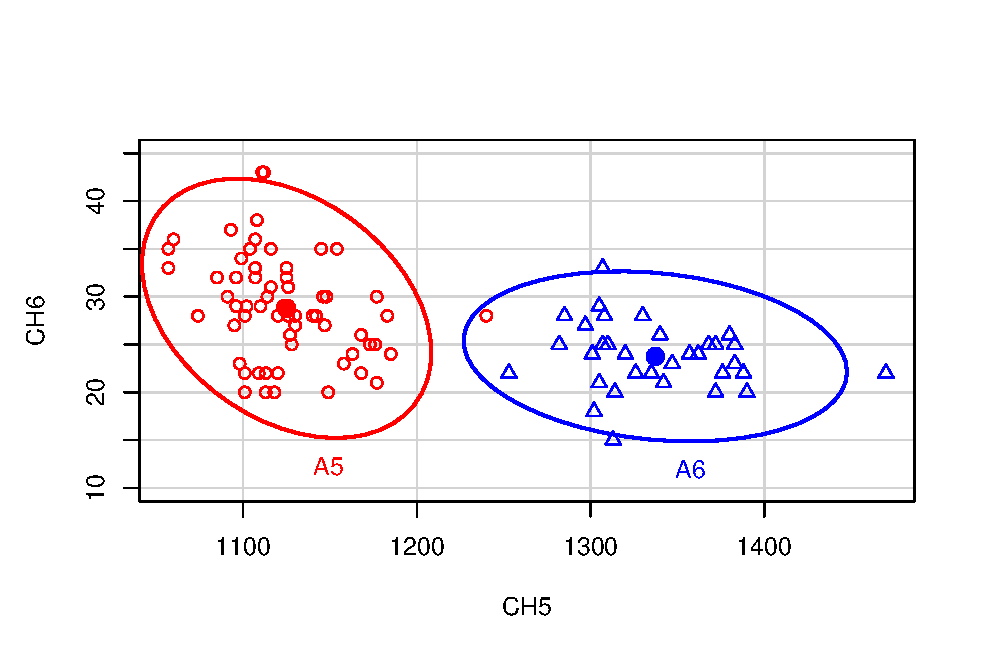
\includegraphics[width = 0.6\textwidth]{ellips.eps}
 	\caption{95\% confidence ellipises for Area 5 and Area 6}
 	\label{ellips}
 \end{figure}


\end{enumerate}

\newpage
\item 
\begin{enumerate}
	\item Display means with Chernoff faces as in Figrue~\ref{faces}.
	\begin{rcode}
#c) Three main regions
#i)Display the Chernoff faces 
 library(TeachingDemos)
 mean_R1 <- sapply(olive_R1[,-1], mean)
 mean_R2 <- sapply(olive_R2[,-1], mean)
 mean_R3 <- sapply(olive_R3[,-1], mean)
 mean_Rs <- cbind(rbind(mean_R1, mean_R2, mean_R3))

faces(mean_Rs, labels = c("R1", "R2", "R3"))
	\end{rcode}
	\begin{figure}[!htb]
		\centering
		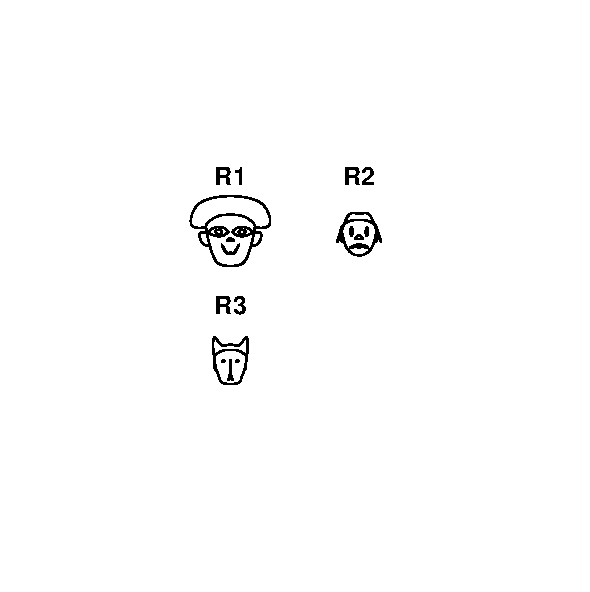
\includegraphics[width = 0.7\textwidth]{faces.eps}
		\caption{Means for 3 big regions}
		\label{faces}
	\end{figure}

According to Chernoff faces, we can see that there is difference in the means among the 3 regions.

\newpage

\item MANOVA for differences in means among 3 regions:
\begin{rcode*}{fontsize = \footnotesize}
#ii) Provide a one-way multivariate analysis of variance.
BigRegions <- rep(0, nrow(olive))
BigRegions[olive$Regions %in% 1:4] <- 1
BigRegions[olive$Regions %in% 5:6] <- 2
BigRegions[olive$Regions %in% 7:9] <- 3
olive <- data.frame(olive, BigRegions = as.factor(BigRegions))
fit.lm <- lm(cbind(CH1, CH2, CH3, CH4, CH5, CH6, CH7, CH8) ~ BigRegions, data = olive)
fit.manova <- Manova(fit.lm)

summary(fit.manova)
\end{rcode*}
The result is
\begin{rcode*}{fontsize = \scriptsize, breaklines = false}

Type II MANOVA Tests:

Sum of squares and products for error:
             CH1         CH2         CH3         CH4         CH5         CH6         CH7
CH1   8712198.47  2068166.15 -591367.187 -16398164.0   6354230.6  -67379.527   74669.446
CH2   2068166.15   951933.35 -239198.820  -5452822.8   3032723.5  -99478.020  -78000.087
CH3   -591367.19  -239198.82  769685.235    808789.9   -875296.2    7021.735   -8832.249
CH4 -16398163.97 -5452822.78  808789.900  44385022.5 -24868011.8  480314.317  266028.691
CH5   6354230.60  3032723.49 -875296.171 -24868011.8  18479382.0 -494033.183 -546173.842
CH6    -67379.53   -99478.02    7021.735    480314.3   -494033.2   66053.027   66956.405
CH7     74669.45   -78000.09   -8832.249    266028.7   -546173.8   66956.405  183120.455
CH8   -143122.66   -59386.98   42218.812    349340.4   -259104.5    9721.942   17177.110
             CH8
CH1  -143122.657
CH2   -59386.983
CH3    42218.812
CH4   349340.368
CH5  -259104.523
CH6     9721.942
CH7    17177.110
CH8    22808.041

------------------------------------------
 
Term: BigRegions 

Sum of squares and products for the hypothesis:
             CH1          CH2          CH3         CH4         CH5          CH6         CH7
CH1   7517535.24  2154506.818  -11358.7365 -16313012.3   4413510.5   466041.967   409500.04
CH2   2154506.82   621547.557   -5516.9112  -4916126.6   1491309.0   135673.062   134446.80
CH3    -11358.74    -5516.911    1273.3995    158440.7   -132434.2    -1874.351   -10109.21
CH4 -16313012.29 -4916126.629  158440.7153  49648363.2 -22971632.2 -1135935.429 -1899371.59
CH5   4413510.54  1491308.999 -132434.1755 -22971632.2  15181902.6   390760.974  1190534.28
CH6    466041.97   135673.062   -1874.3508  -1135935.4    390761.0    29981.812    34226.86
CH7    409500.04   134446.801  -10109.2121  -1899371.6   1190534.3    34226.860    94004.06
CH8    823641.31   235143.784    -739.1389  -1733475.8    432963.5    50590.072    41048.13
              CH8
CH1   823641.3147
CH2   235143.7841
CH3     -739.1389
CH4 -1733475.8370
CH5   432963.5194
CH6    50590.0723
CH7    41048.1276
CH8    90443.6429

Multivariate Tests: BigRegions
                 Df test stat approx F num Df den Df     Pr(>F)    
Pillai            2  1.593690 276.0350     16   1126 < 2.22e-16 ***
Wilks             2  0.031702 324.3008     16   1124 < 2.22e-16 ***
Hotelling-Lawley  2 10.816547 379.2552     16   1122 < 2.22e-16 ***
Roy               2  8.494086 597.7713      8    563 < 2.22e-16 ***
---
Signif. codes:  0 ‘***’ 0.001 ‘**’ 0.01 ‘*’ 0.05 ‘.’ 0.1 ‘ ’ 1
\end{rcode*}

From the result we can see the p-value is small, and we conclude that there are differences in means among the 3 main regions.


\end{enumerate}





		\end{enumerate}

	
 	\end{enumerate}









	
	
	
	\end{document}